\documentclass[11pt]{article}

%-----------------------------------------------------------------------------
% PDF setup
%-----------------------------------------------------------------------------
%\usepackage{thumbpdf}
%\usepackage[pdftex]{graphicx}
%\usepackage[pdftex]{color} % black,white,red,green,blue,cyan,magenta,yellow
%\definecolor{myBlue}{rgb}{0.0,0.0,0.55}
%\usepackage[pdftex,colorlinks=true,citecolor=myBlue,linkcolor=myBlue]{hyperref}

%-----------------------------------------------------------------------------
% Additional packages
%-----------------------------------------------------------------------------
%\usepackage{multibib}
\usepackage{amsfonts}
\usepackage{amsthm}
\usepackage{amsmath}
\usepackage{enumerate}
\usepackage{graphicx}
\usepackage{color}      % colored text, See "Graphics and Colour with LaTeX" by Patrick W. Daly
%\usepackage{subfigure}
\usepackage{psfrag}
%\usepackage[nottoc,notbib,notindex,notlot,notlof]{tocbibind}

%-----------------------------------------------------------------------------
% Dimensions
%-----------------------------------------------------------------------------
\setlength{\parindent}{2em} \setlength{\parskip}{0pt}
\setlength{\headheight}{0.0in} \setlength{\headsep}{0.0in}
\setlength{\headsep}{0.0in} \setlength{\topmargin}{0.0in}
\setlength{\textheight}{9.2in} %%% 8.66in = 220mm
\setlength{\textwidth}{6.6in}  %%% 6.50in = 165mm
\setlength{\evensidemargin}{0.0in}
\setlength{\oddsidemargin}{-0.15in}
\def\linespacing#1{\renewcommand{\baselinestretch}{#1}\small\normalsize}

%-----------------------------------------------------------------------------
% Symbols
%-----------------------------------------------------------------------------
\def\tbar{|\hspace*{-0.15em}|\hspace*{-0.15em}|}
\def\Ahatstar{{}^{*}\!\!\hat{A}}
\def\bold#1{{\bf #1}}
\def\text#1{{\rm #1}}
\def\calg#1{{\cal #1}}
\def\bbbb#1{{\mathbb #1}}
\def\PLTMG{{\sc PLTMG}}
\def\MC{{\sc MC}}
\def\MCX{{\sc MCX}}
\def\MALOC{{\sc MALOC}}
\def\SG{{\sc SG}}
\def\MCLAB{{\sc MCLab}}
\def\APBS{{\sc APBS}}
\def\FETK{{\sc FE}{\small tk}}
\newcommand{\half}{\frac{1}{2}}
\newcommand{\Lapse}{N}                  %Lapse function
\newcommand{\hme}{\hat g}               %background metric
\newcommand{\hnabla}{\hat \nabla}       %background covariant derivative
\newcommand{\hGamma}{\hat \Gamma}       %background Christoffel
\newcommand{\Shift}{X}                  %Shift Vectorfield
\newcommand{\Lie}{{\mathcal L}}         %Lie derivative
\newcommand{\del}{\delta}               %gauge quantity
\newcommand{\tr}{{\text{\rm tr}}}       %trace
\newenvironment{enumerateX}
{\begin{list}{\arabic{enumi}.}{
     \usecounter{enumi}
     \leftmargin 2.0em\topsep 0.2em\itemsep -0.2em\labelwidth 50.0em}}
{\end{list}}
\newenvironment{itemizeX}
{\begin{list}{\labelitemi}{
     \leftmargin 2.0em\topsep 0.2em\itemsep -0.2em\labelwidth 50.0em}}
{\end{list}}
%\newenvironment{listX}
%{\begin{list}{}{
%     \leftmargin 2.0em\topsep 0.2em\itemsep -0.2em\labelwidth 50.0em}}
%{\end{list}}
%\newtheorem{lemma}{Lemma}
%\newtheorem{theorem}{Theorem}
%
%\newcommand{\RR}{{\mathbb{R}}}
%\newcommand{\ynder}{{\partial_\nu y}}
%\newcommand{\pnder}{{\partial_\nu p}}
%\newcommand{\domain}{\Omega}
%\newcommand{\bound}{\Gamma}
%\newcommand{\nablab}{{\nabla_{\bound}}}
%
%\newcommand{\vX}{\vec{X}}
%\newcommand{\vk}{{\vec \kappa}}
%\newcommand{\vn}{{\vec\nu}}
%\newcommand{\vV}{{\vec V}}
%\newcommand{\vh}{{\vec h}}

%-----------------------------------------------------------------------------
% Macros for notes
%---------------------------------
 \newcommand{\mnote}[1]{{\marginpar{\raggedright\tiny\em
     $\!\!\!\!\!\!\,\bullet$ #1}}} % enable marginal notes
 \newcommand{\tnote}[1]{{#1}}      % enable text notes
%---------------------------------
%\newcommand{\mnote}[1]{{}}        % disable marginal notes
%\newcommand{\tnote}[1]{{}}        % disable text notes
%-----------------------------------------------------------------------------

\newcommand{\vnode}[1]{\psfrag{v#1}{$V_{#1}$}}
\newcommand{\eedge}[1]{\psfrag{e#1}{$E_{#1}$}}
\newcommand{\ttri}[1]{\psfrag{t#1}{$T_{#1}$}}

%-----------------------------------------------------------------------------
% Proposal body
%-----------------------------------------------------------------------------

\newcounter{savecount}
\begin{document}

\linespacing{1.0}

%bisection diagram

\section{Bisection Diagrams}

\subsection{2-D Bisection of Terminal Triangle Pair}

\begin{figure}
\begin{center}

\vnode{0} \vnode{1} \vnode{2}
\psfrag{vh}{$\widehat{V}$}

\psfrag{longedge}{(longest edge)}

\psfrag{ar1}{\Huge{$\Downarrow$}}
\psfrag{ar2}{\Huge{$\Rightarrow$}}

\psfrag{t0}{$t_0$}
\psfrag{t1}{$t_1$}
\psfrag{s0}{$s_0$}
\psfrag{t0d}{$\tilde{t}_0$}

\psfrag{A}{$A$}
\psfrag{B}{$B$}
\psfrag{C}{$C$}
\psfrag{D}{$D$}

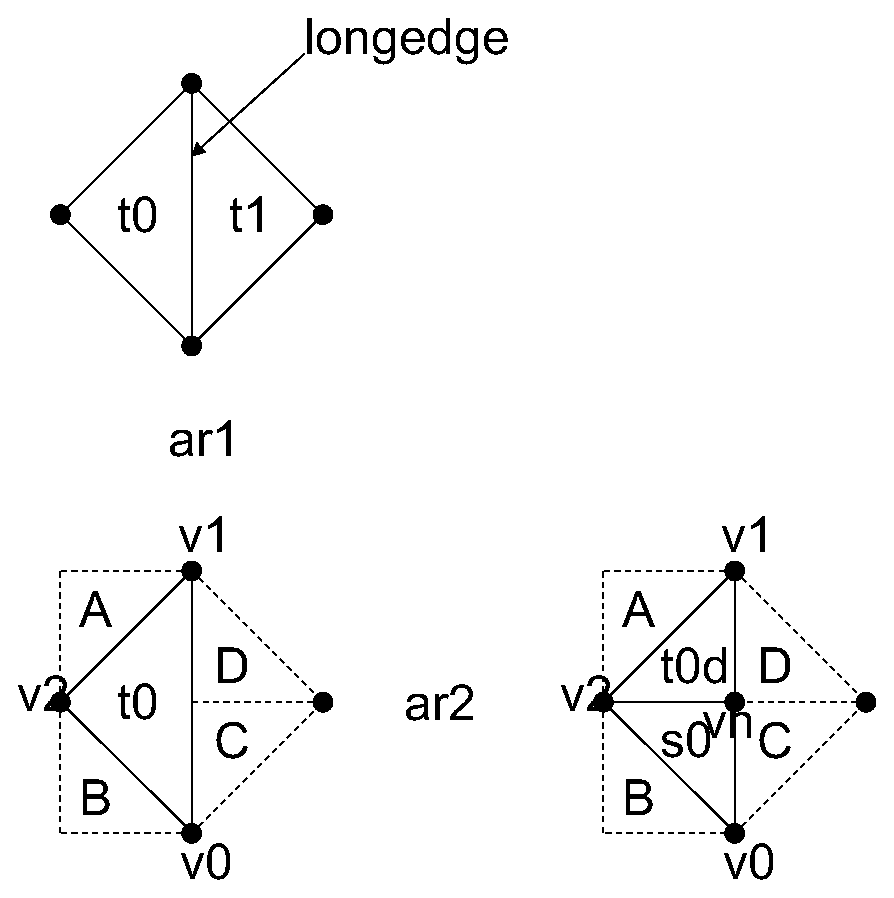
\includegraphics[width=4.0in]{Bisect_Terminal_Triangle_Pair}
\caption{Diagram of bisection process for terminal triangle pair.  The initial pair consists of two triangles $t_0, t_1$ that share a longest edge.  The initial neighbors of $t_0$ are the triangles labeled $A, B, t_1$.  Assuming that $t_1$ has already been bisected into triangles $C, D$, we see an intermediate stage for bisecting $t_0$.  We then replace $t_0$ by triangles $\tilde{t}_0$ and $s_0$ whose neighbors are adjusted accordingly.} \label{fig:Bisect_Terminal_Pair_2D}
\end{center}
\end{figure}

Assume we are given a terminal pair of triangles that share a longest edge (see Figure \ref{fig:Bisect_Terminal_Pair_2D}).  Bisecting the longest edge adds a new vertex with global index denoted $\widehat{V}$.  To better explain the bisection of the adjacent triangles, we assume that $t_1$ is already bisected into two triangles labeled $C, D$.

To bisect the triangle $t_0$, we must replace the triangle connectivity data of $t_0$ with the connectivity data of $\tilde{t}_0$, followed by adding a new triangle to the mesh, namely $s_0$. We then change the neighbors of $t_0$ to those of $\tilde{t}_0$, and add the neighbors of $s_0$ to the neighbor list.  Finally, we adjust the neighbors of $A$ and $B$ to correctly correspond to the new mesh.  This is summarized as follows.
\begin{equation}\label{eqn:tri_connectivity_and_neighbors}
\begin{split}
    \text{triangle~connectivity~of} ~\tilde{t}_0 &= [\widehat{V}, V_1, V_2], \quad \text{neighbor~connectivity~of} ~\tilde{t}_0 = [A, s_0, D] \\
    \text{triangle~connectivity~of} ~s_0 &= [\widehat{V}, V_2, V_0], \quad \text{neighbor~connectivity~of} ~s_0 = [B, C, \tilde{t}_0]
%    \text{neighbor~connectivity~of} ~\tilde{t}_0 &= [A, s_0, D] \\
%    \text{neighbor~connectivity~of} ~s_0 &= [B, C, \tilde{t}_0]
\end{split}
\end{equation}

Note that the global triangle index of $t_0$ and $\tilde{t}_0$ is identical, since we simply \emph{replaced} $t_0$ by $\tilde{t}_0$.  This means that the neighbor data for triangle $A$ does not need to be changed.  However, we must update the neighbors of triangle $B$, i.e. if $B$'s $k$th neighbor was $t_0$ before the bisection, then $B$'s $k$th neighbor after bisection should be $s_0$.

Note: the process for bisecting $t_1$ is exactly the same as for $t_0$; just rotate the diagrams in Figure \ref{fig:Bisect_Terminal_Pair_2D} by $180^\circ$.  In other words, triangle $C$ is really $\tilde{t}_1$, and $D$ is $s_1$.



%%%%%%


%%--------------------------------------------------------------------
%% References
%%--------------------------------------------------------------------
%
%\vfill\eject
%\setcounter{page}{1}

\end{document}
